\begin{figure}[H]
  \centering
  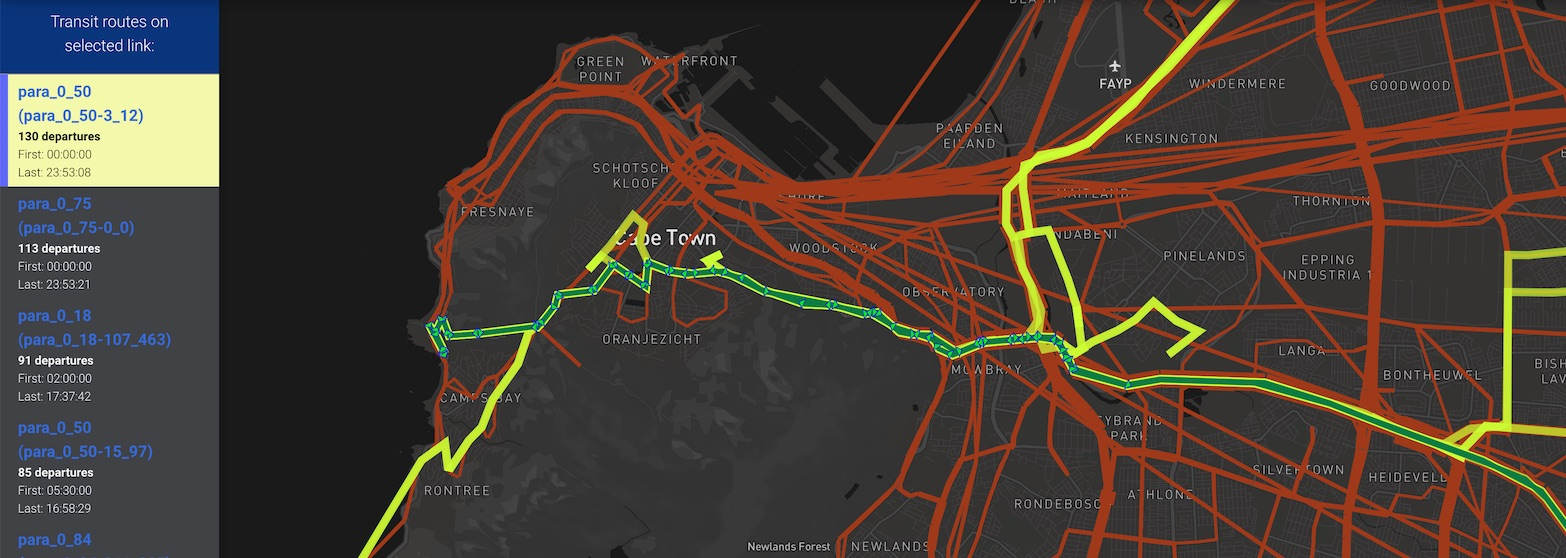
\includegraphics[width=0.8\textwidth]{assets/transit.jpg}
  \caption{Transit routes and ridership}
\end{figure}

This visualization depicts transit routes and lines, and can also display ridership data if available.

\hypertarget{usage}{%
\subsection{Usage}}

No YAML is required. If the run folder contains a
\texttt{*output\_transitSchedule.xml.gz} file, then this view will be
available and the transit route supply can be explored.

If the run folder also contains
\texttt{*pt\_stop2stop\_departures.csv.gz} then the transit ridership
(demand) will also be loaded. This may take a few moments to load.

\hypertarget{exploring-transit}{%
\subsubsection{Exploring transit}\label{exploring-transit}}

Click on any transit link to see the list of transit routes which
traverse that link. You can select any individual route from the details
panel to see the extent of the route.
